\documentclass[../main.tex]{subfiles}
\graphicspath{{\subfix{../Figures/}}}

\begin{document}

\chapter{Experiments}

We now present our three experiments aiming to address the problems stated in \autoref{ch:methods}.

First we give details on settings common to all experiments.

\section{Models}

All models are trained using the Adam algorithm \cite{kingmaAdam2014} with a learning rate of $1 \times 10^{-3}$.

\subsection{Classifier}
\label{exp/classifiers}

The classifier architecture in our analyses is an MLP consisting of two 50-node linear layers each followed by a $\relu$, then one last linear layer outputting $\outputdim$ logits.

In \autoref{fig:confusion_matrices} we show the test predictions of our classifier architecture, trained on each dataset with the batch size given in \autoref{tab:datasets}.
\begin{figure}
    \centering
    \begin{subfigure}[b]{0.4\textwidth}
        \centering
        \includegraphics[width=\textwidth]{./confusion_matrices/cake_on_sea/confusion_matrix_svg-tex.pdf}
        \caption{Accuracy on \CakeOnSea.}
\label{fig:cos_confusion_matrix}
    \end{subfigure}
    % \hfill
    \begin{subfigure}[b]{0.4\textwidth}
        \centering
        \includegraphics[width=\textwidth]{./confusion_matrices/forest_cover/confusion_matrix_svg-tex.pdf}
        \caption{Accuracy on \ForestCover.}
        % \label{fig:three sin x}
    \end{subfigure}

    \begin{subfigure}[b]{0.4\textwidth}
        \centering
        \includegraphics[width=\textwidth]{./confusion_matrices/wine_quality/confusion_matrix_svg-tex.pdf}
        \caption{Accuracy on \WineQuality.}
        % \label{fig:y equals x}
    \end{subfigure}
    % \hfill
    \begin{subfigure}[b]{0.4\textwidth}
        \centering
        \includegraphics[width=\textwidth]{./confusion_matrices/online_news_popularity/confusion_matrix_svg-tex.pdf}
        \caption{Accuracy on \OnlineNewsPopularity.}
        % \label{fig:three sin x}
    \end{subfigure}

    \caption{Accuracy of our MLP classifier on each dataset.}
    \label{fig:confusion_matrices}
\end{figure}

It seems the classifier achieves low accuracy on \WineQuality{} and \OnlineNewsPopularity{} in particular.
These datasets are originally designed for regression, so they are perhaps not well adapted to classification; however, their size is also likely a factor: they have on the order of $10^2$ training examples per dimension where the others have on the order of $10^4$.

All datasets also have significant class imbalance: in \ForestCover{} the test set contains 56382 points with true class 1 while only 554 points in class 3.

\subsection{Autoencoder}

We build a normalizing flow model according to the NICE architecture described in \autoref{bg/nf} \cite{dinhNICE2015}.
The model is trained according to a Gaussian prior distribution, and its layers are 4 additive coupling layers where we divide the input into the odd columns and the even columns, and the nonlinearity is an MLP with 2 layers of 20 nodes each.

\section{Experiment 1: Validity losses}

In this experiment, we seek to determine the validity loss that maximizes validity rate among a number of choices.
For this we measure the validity rate over CFs generated from the test set across several CF methods and losses.

\paragraph{Description}
\label{validity_losses/description}

For a given dataset, we train one classifier.
Then for this dataset, we train several autoencoders all with the same architecture and with different seeds to average out random effects due to model initialization and dataset train-test split.
The seeds are generated uniformly based on one primary seed.

For a given dataset, we measure the validity rate across the whole test set.
That is, for every test point, we run the classifier to get the $\source$ class ($\source = \arg\max_{c \in \setclasses} f(x)$), and we sample the target class uniformly from $\setclasses \backslash \{\source\}$.
Then we generate a path using the given loss $\lossval$, and count it as valid or not.
It is important to sample the $\target$ uniformly to get a full understanding because, even though the label distribution might not be uniform, in general there is no reason to prefer explanations for a given target rather than another.

We average the rates over the different seeds, and report the standard error.

\paragraph{Baselines}

The methods we use to produce the paths are variations on \ls{} and \revise{}.
Specifically, we run both methods twice: once with regularization on the $L_1$ distance, with $\lambda_\text{distance} = 0.3$ and one without regularization (with $\lambda_\text{distance}$ set to 0).
In the future using some automatic tuning procedure would be preferable: in our case $\lambda_\text{distance} = 1$ led to immobile paths whereas $\lambda_\text{distance} = 0.3$ might be too close to regularization at all.

In fact, our implementation of both \ls{} and \revise{} is a joint abstraction that takes a parameter for the frequency of the gradient computation: for \revise{} this is set to 1 (\ie{} recompute the gradient after every step) while for \revise{} it is null (\ie{} never recompute it).
This way the number of steps and step size can be set to the same values with confidence.
However, this means that we do not run \revise{} using a more sophisticated optimization algorithm like \method{Adam} or \method{RMSprop}.

The losses compared in this experiment are as follows:
\begin{itemize}
    \item The probability-based losses: $\PrbTarget, \PrbSource{}$
    \item The log-probability-based losses: $\LogPrbTarget, \LogPrbSource{}, \LogPrbOthers{}$
    \item The logit-based losses: $\LogitTarget, \LogitSource{}, \LogitOthers{}$
\end{itemize}
where we test all losses that can be parametrized with the default parameter of $\lambda = 1$ and also with $\lambda = 0.1$, for a total of 13 losses ($\PrbTarget$ is not parametrized, and recall that $\PrbOthers{}$ is equivalent to $\PrbTarget$.).
Here again, a larger scale parameter search could have been interesting, but instead we first select the best-performing loss and then show the progression for $\lambda \in [0, 1]$.

\paragraph{Datasets}

We run our experiment on the datasets described in \autoref{sec:datasets}, namely \CakeOnSea, \ForestCover, \WineQuality{} and \OnlineNewsPopularity.

The batch sizes are chosen so that one epoch takes less than 10 steps, except for \ForestCover{} where the size of the train set would have made very large batches.
The final numbers are:
\begin{itemize}
    \item \CakeOnSea: 12000
    \item \ForestCover: 25000
    \item \WineQuality: 500
    \item \OnlineNewsPopularity: 3000
\end{itemize}

\paragraph{Metrics}

The one metric in this experiment is the validity rate, \ie{} the proportion of paths that reach their target class across the whole test set.

\paragraph{Results}

The results for each dataset and loss are given in \autoref{tbl:validity_losses}.
We highlight in gray the five losses that yield the best average validity rate across all path methods; the results are not uniform across datasets so we resort to this rough estimate to decide between the losses.

\begin{table}[h!]
\centering
\subfile{../Figures/validity_losses.tex}
\caption{Validity rate means with their standard error. Highlighted are the five losses with the best average results.}
\label{tbl:validity_losses}
\end{table}

As expected, the validity rate achieved by \revise{} is generally much more acceptable than that of \ls{}, across all losses.
It would seem $\LogitSource{}$ is always among the best validity losses. However, it is not always clear which value of $\lambda$ should be used.
Hence, we show the validity rate for several values of $\lambda$ in \autoref{fig:lambda_progression}.

\begin{figure}[htbp]
    \centering
    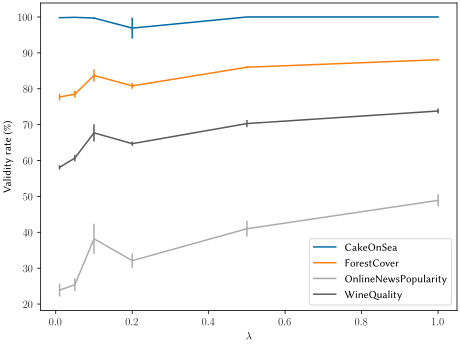
\includegraphics[width=0.7\textwidth]{./logit_source_lambda_progression}

    \caption{Validity rate for $\LogitSource{\lambda}$ for different values of $\lambda$.}
    \label{fig:lambda_progression}
\end{figure}

To make better sense of our findings, we also plot our various losses and their gradients on \CakeOnSea.
The plots are shown in full in \autoref{fig:cf_losses_all} and \autoref{fig:cf_gradients_all}.
Here, we select plots for some losses and where the target class is always class 2.


\begin{figure}[htbp]
    \centering
    \includegraphics[width=\textwidth]{./cf_losses/cf_losses_detail}
    \caption{Loss profile for various losses on \CakeOnSea, with ${\target = 2}$.}
    \label{fig:cf_losses_detail}

    \vspace*{\floatsep}% https://tex.stackexchange.com/q/26521/5764

    \includegraphics[width=\textwidth]{./cf_losses/cf_gradients_detail}
    \caption{Opposite of the loss gradient for various losses on \CakeOnSea, with $\target = 2$.}
    \label{fig:cf_gradients_detail}
\end{figure}

\paragraph{Interpretation}

From the test accuracy of our classifier which we showed in \autoref{fig:cos_confusion_matrix}, we know that the prediction probabilities are all close to 1, except near the decision boundaries of course.
Hence, we can verify our intuitive thinking from \autoref{sec:validity_losses}: for the probability-based losses, the loss is very flat, \ie{} the gradient is close to zero.
For $\LogPrbOthers{}$ it seems the logits from the other classes counteract the target logit, so that paradoxically the paths get pushed away from class 2 in places.
For the logit-based losses however, the behavior is fairly uniform across the whole data distribution, and so the gradients clearly point the path towards class 2.

This leads us to choose $\LogitSource{\lambda=1}$ as validity loss in the rest of our analyses.

\section{Experiment 2: Path regularized training}
\label{exp/path_reg}

Having determined an appropriate validity loss to use for generating valid paths, we turn now to our objective of interpretability.
In this experiment we seek to determine if \ls{} equipped with a path regularized autoencoder can perform on the same level as \revise{}, increasing interpretability without compromising validity.

Our proxy for complexity of a path is \emph{the number of class boundary crossings}:
the path should ideally transition from $\source$ to $\target$ without going through other classes.
We thus add our $\BoundaryCrossLoss$ to the $\nll$ when computing the loss of the autoencoder.
Our final loss for training the autoencoder is
\begin{align*}
    \loss(\phi) = \nll(\phi) + \BoundaryCrossLoss(\apath)
\end{align*}
where $\apath$ is a path generated with some CF method.


\paragraph{Description}

First, we generate some seeds.
For a given dataset, we train one classifier, as in \autoref{validity_losses/description}.
For each seed, we train several autoencoders: one without path regularization, and then one per CF generation method using the path regularized training procedure.

Then, each autoencoder is used to produce explanation paths on the whole test set, like in \autoref{validity_losses/description}, and metrics are computed with the paths as input.
Finally, for each explanation method, we aggregate the metrics obtained for each seed and report the standard error.

The paths are 100 points long (including the starting point, so the number of steps is 99) and the step size $\lambda_\text{LS}$ is 0.1. We found this to be satisfactory so that the path is long enough to reach the target class, yet with step size short enough that the path does not go too far too quickly.

\paragraph{Baselines}
\label{exp/path_reg/baselines}

Since the distance parameter seems inconsequential from our previous results,
in this experiment we use \ls{} and \revise{} in their basic form, \ie{} with no distance regularization for \ls{} and with $\lambda_\text{distance} = 0.3$ for \revise.

\paragraph{Datasets}

For memory performance reasons we adapt the batch size for each dataset.
We compute the batch size so that one training epoch (one pass through $\trainset$) takes 20 steps, except for \ForestCover{} where the batches are still too big.
The final numbers are:
\begin{itemize}
    \item \CakeOnSea: 2881
    \item \ForestCover: 5000
    \item \WineQuality: 195
    \item \OnlineNewsPopularity: 1190
\end{itemize}

\paragraph{Metrics}

We measure the validity rate, as before, as well the number of boundary crossings \emph{before reaching $\target$} (so if the path goes directly from $\source$ to $\target$ the value is 0) which is the proxy for interpretability we chose.

For measuring realism, we use a specially-trained autoencoder with the same architecture as the others, trained using only the $\nll$ as a loss.
The realism score for $\CF{x}$ is given by its $\nll$ as computed by our special autoencoder.

We also measure the computational complexity (the duration for one computing one step of one path).

\subsection{Results}

\subsection{Interpretation}

\section{Experiment 3: Robustness of explanations with path regularization}

Given that we were able to achieve more interpretable paths using path regularization, we ask whether it is possible to meet any interpretability criterion, even a nonsensical one.
For example, can we use path regularization so that all paths pass through one designated point, regardless of $x$ and $\target$?
To do so, we select a point $\xgoal \in \inputspace$ that we can reasonably expect to be unrealistic, but is not completely out of reach compared to points in the train set.
Then, we devise a path loss that encodes the distance from a path to $\xgoal$, and let our path regularization training enforce this constraint.

\paragraph{Description}

We perform path regularized training using the adversarial path loss described in \autoref{methods:robustness}.
The loss encodes how close a path passes by a given point $\xgoal$, which is potentially unrealistic.
In our experiment, we pick a $\xgoal$ that is easy to compute, likely unrealistic yet not completely out of bounds for the dataset:
\begin{equation}
    \xgoal = (\max\{ x_i : x \in \trainset \})_{i=1}^D
\end{equation}
\ie{} $\xgoal_i$ is the largest value encountered in the dataset for feature $i$.

Apart from this the setup is the same as that described in \autoref{exp/path_reg}, where we compare paths with the distance path regularization and without.

\paragraph{Baselines}

We use the same baselines as in the previous experiment (\autoref{exp/path_reg/baselines}).

\paragraph{Datasets}

We use the same datasets as in the previous experiments.

\paragraph{Metrics}

As before, we analyze the trade-off that is incurred by applying path regularization.
We measure the validity rate, as well as the realism score and the path loss.

Since we seek to minimize the distance from a path to $\xgoal$, we  include our path distance loss as a measure.
Yet, it is important that manipulated paths retain the validity quality for the attack to be successful, hence we measure validity as well.

\paragraph{Results}

\paragraph{Interpretation}



\end{document}